\section{Two-Stage Calibration}
\label{sec:estimation}

\subsection{Identification Strategy}

The model has three parameters: $\theta = (\alpha_\nu, \sigma_\nu, \kappa)$, where $(\hat{\alpha}_\nu, \hat{\sigma}_\nu)$ govern the capital supply distribution $\hat{\nu} \sim \text{LogNormal}(\hat{\alpha}_\nu, \hat{\sigma}_\nu^2)$, and $\kappa$ scales deadweight bankruptcy costs. The calibration proceeds in two stages — not as a joint SMM estimator. The primary empirical evidence for the model's central prediction comes from the within-firm panel regression in Section~\ref{sec:results}; the calibration here provides structural quantities (debt capacity bounds, spread lower bounds) that are consistent with that reduced-form evidence.

\paragraph{Identification of $(\alpha_\nu, \sigma_\nu)$: FRED-anchored calibration.}
I calibrate the capital supply distribution $\hat{\nu}$ by anchoring it to aggregate credit market data. The primary external anchor is the FRED Flow-of-Funds series for credit market instruments held by the US financial sector: the cross-sectional Fr\'{e}chet mean of firm cash-flow distributions correlates $0.87$ with this Federal Reserve series over 1989--2024 (Figure in Appendix~\ref{app:distribution_robustness}). This high correlation establishes that the Fr\'{e}chet mean is not a mechanical artifact of the cross-section of firms it explains, but a valid proxy for an independently observable aggregate capital supply distribution measured by the Federal Reserve outside the Compustat sample. I use the Fréchet mean operationally (as it avoids direct leverage-data contamination) validated against FRED as the primary identification anchor. The approach avoids circularity: if $\hat{\nu}$ were estimated from bond issuance volumes or spreads, the Wasserstein distance $\widehat{W}_1(\hat{\mu}_{it}, \hat{\nu})$ would be jointly determined with the leverage it is supposed to explain. The parameters $(\hat{\alpha}_\nu, \hat{\sigma}_\nu)$ come from fitting a LogNormal approximation to the Fr\'{e}chet-mean quantile function.

\textit{Circularity concern and its resolution.} A natural concern is that $\hat{\nu}$, defined as the Fréchet mean of the firm distributions, makes $\widehat{W}_{1,\text{shape}}$ a mechanical outlier-distance measure: a firm scores high simply for being an unusual element of the cross-section. Three features address this, ordered by their persuasive weight. First, and most directly, the Fr\'{e}chet-mean quantile function correlates $0.87$ with FRED Flow-of-Funds debt supply aggregates computed independently from the Compustat sample (Appendix~\ref{app:distribution_robustness}). This confirms that the cross-sectional barycenter tracks an independently observable capital supply object — not a statistical artifact of the leverage data it is used to explain. The $0.87$ correlation holds across 1989--2024 including the 2008--09 contraction and the 2020 COVID shock. Second, the equilibrium interpretation provides theoretical grounding: the Fr\'{e}chet mean in Wasserstein space is the population average distribution under the competitive equilibrium in Appendix~\ref{app:tradeoff_special_case}, where free entry and zero-profit conditions imply that aggregate capital supply available to any one firm converges to the cross-sectional barycenter in the large-market limit. Third, the within-firm result (column 5 of Table~\ref{tab:panel_regressions}) cannot be explained by a mechanical-outlier story: if $\widehat{W}_{1,\text{shape}}$ only flagged structurally unusual firms, its within-firm variation would be near zero and would not predict changes in leverage over time for the same firm.

\paragraph{Calibration of $r_f$.}
The risk-free rate $r_f$ in the lender participation constraint~\eqref{eq:pc} is calibrated as the sample-period average 3-month US Treasury bill rate (FRED series TB3MS) over 2012--2024: $\hat{r}_f = 0.020$ (2.0\%). This is estimated directly from the data rather than normalized to zero; the calibrated value changes the equilibrium borrowing scale $\hat{\lambda}_{it}^*$ only marginally (by construction, since $\hat{r}_f$ is small) but ensures the participation constraint is correctly specified.

\paragraph{Identification of $\kappa$ via SMM spread moment conditions.}
Given $(\hat{\alpha}_\nu, \hat{\sigma}_\nu)$, the bankruptcy cost parameter $\kappa$ is identified from the 10 decile-mean credit spread moments jointly, treating Proposition~\ref{prop:spreads}'s inequality as a binding moment condition. The model predicts that for each $\widehat{W}_{1,\text{shape}}$ decile $d$,
\begin{equation}
  \bar{s}_d \;\geq\; \hat{\kappa}\,\frac{\bar{W}_{1,\text{shape},d}}{2\,\hat{\mathbb{E}}_\nu[Y]}\times 10{,}000\quad\text{bps},
  \label{eq:smm_moment}
\end{equation}
where $\bar{s}_d$ is the mean TRACE spread in decile $d$ and $\bar{W}_{1,\text{shape},d}$ is the mean $\widehat{W}_{1,\text{shape}}$ of bond-issuing firms in that decile. The SMM estimator maximizes $\kappa$ subject to all 10 inequality constraints simultaneously:
\begin{equation}
  \hat{\kappa} \;=\; \min_{d\in\{1,\ldots,10\}}\;\frac{\bar{s}_d\,\cdot\,2\,\hat{\mathbb{E}}_\nu[Y]}{\bar{W}_{1,\text{shape},d}\times 10{,}000}.
  \label{eq:kappa_smm}
\end{equation}
This identifies $\hat{\kappa}$ as the tightest value consistent with the proposition's lower bound holding for all decile moments simultaneously. The binding constraint is decile 9 --- where the model lower bound exactly matches the observed mean spread of $169.7$ bps for high-mismatch investment-grade bond issuers. Under $\hat{\kappa}=0.104$, the lower bound is satisfied for all ten deciles with zero violations; the largest slack occurs at decile 1 (data: $462$ bps, model: $53$ bps) where the composition of investment-grade issuers with non-model spread premia generates the largest gap. This avoids the sign-reversal problem that arises from the OLS coefficient on TRACE spreads, which is negative due to compositional selection of bond issuers across the $\widehat{W}_{1,\text{shape}}$ distribution.

\paragraph{Within-firm spread test.}
As a complementary exercise, I estimate a within-firm regression of TRACE credit spreads on $\widehat{W}_{1,\text{shape}}$, including firm and year-quarter fixed effects. The coefficient is $-1{,}316$ bps (s.e.\ $1{,}162$, $t = -1.13$, $N = 23{,}814$ firm-quarters, 1,035 firms), statistically insignificant. This non-result reflects a power problem, not a failure of the model. Within the TRACE subsample, the within-firm standard deviation of $\widehat{W}_{1,\text{shape}}$ is approximately $0.003$ — nearly two orders of magnitude smaller than the cross-sectional SD of $0.075$ used in the panel regression. A bond-issuing firm's cash flow distribution shape does not vary sufficiently within-firm over 2012--2024 to identify a within-firm spread effect. The 95\% confidence interval for the within-firm estimate ($-3{,}594$ to $+962$ bps) is wide enough to encompass the cross-sectional slope of $-4{,}243$ bps. The theoretically appropriate test of Proposition~\ref{prop:spreads} is therefore the cross-sectional comparison of model spread lower bounds against actual decile mean spreads (Table~\ref{tab:decile_fit}), not a within-firm estimator that cannot identify the relevant variation.

\paragraph{Wasserstein distance computation.}
Given $(\hat{\alpha}_\nu, \hat{\sigma}_\nu)$, the Wasserstein-1 distance for firm-quarter $(i,t)$ is approximated on the ten-point discretization:
\begin{equation}
  \widehat{W}_1(\hat{\mu}_{it}, \hat{\nu}) = \frac{1}{10}\sum_{k=1}^{10}|\hat{q}_{it,k} - \hat{Q}_\nu(u_k)|,
  \label{eq:w1_approx}
\end{equation}
where $\hat{Q}_\nu(u_k) = \exp(\hat{\alpha}_\nu + \hat{\sigma}_\nu\Phi^{-1}(u_k))$ is the quantile function of $\hat{\nu}$ at level $u_k$. This is the exact $W_1$ on the ten-point empirical measure of $\hat{\mu}_{it}$. I also compute the shape component:
\begin{equation}
  \widehat{W}_{1,\text{shape}}(\hat{\mu}_{it}, \hat{\nu}) = \frac{1}{10}\sum_{k=1}^{10}\bigl|(\hat{q}_{it,k} - \hat{\mathbb{E}}_{\mu_{it}}[X]) - (\hat{Q}_\nu(u_k) - \hat{\mathbb{E}}_\nu[Y])\bigr|,
\end{equation}
which removes the mean difference and isolates the higher-moment (shape) mismatch. Proposition~\ref{prop:leverage_wasserstein} applies conditional on equal means; $\widehat{W}_{1,\text{shape}}$ is the empirically relevant object when comparing firms with different average cash flow levels.

\subsection{Structural Parameter Estimates}

Table~\ref{tab:structural} reports the parameter estimates. Standard errors for $(\hat{\alpha}_\nu, \hat{\sigma}_\nu, \hat{\mathbb{E}}_\nu[Y])$ are from 500 Compustat firm-level bootstrap replications. The standard error for $\hat{\kappa}$ is from 500 TRACE firm-level bootstrap replications: for each replication, TRACE bond-issuing firms are resampled with replacement, decile-mean spreads and $\bar{W}_{1,\text{shape},d}^{\text{spr}}$ are recomputed, and $\hat{\kappa}$ is re-solved from \eqref{eq:kappa_smm}.

\begin{table}[htbp]
\centering
\caption{Structural Parameter Estimates}
\label{tab:structural}
\begin{threeparttable}
\begin{tabular}{lcc}
\toprule
Parameter & Estimate & Bootstrap SE \\
\midrule
$\hat{\alpha}_\nu$ (log-location of $\hat{\nu}$) & -3.4926 & (0.0132) \\
$\hat{\sigma}_\nu$ (log-scale of $\hat{\nu}$) & 2.3919 & (0.0025) \\
$\hat{\kappa}$ (bankruptcy cost scale) & 0.1039 & (0.0049) \\
\midrule
\multicolumn{3}{l}{\textit{Implied moments of $\hat{\nu}$}} \\
$\mathbb{E}_{\hat{\nu}}[Y]$ (mean capital endowment, 10-pt empirical) & 0.0903 & (0.0096) \\
$\text{Std}(\hat{\nu})$ & 9.2729 & (---) \\
\midrule
\multicolumn{3}{l}{\textit{Identification}} \\
$R^2$ (LogNormal fit to $\hat{\nu}$) & 0.4218 & --- \\
Binding decile (kappa SMM) & D9 & --- \\
$R^2$ (leverage decile fit) & -10.9473 & --- \\
Spearman $\rho$ (lev.\ vs.\ $W_1$ decile) & 0.4545 & ($p=0.187$) \\
\bottomrule
\end{tabular}
\begin{tablenotes}
\small
\item Bootstrap standard errors (500 firm-level replications) in parentheses.
$\hat{\nu} \sim \text{LogNormal}(\hat{\alpha}_\nu, \hat{\sigma}_\nu^2)$ is the
Fr\'{e}chet mean of firm cash-flow distributions.
$\hat{\kappa}$ is identified via SMM bound-tightening (Equation~\ref{eq:kappa_smm}),
binding at decile D9. Bootstrap SE for $\hat{\kappa}$
is from 500 replications resampling TRACE bond-issuing firms.
Sample: Compustat quarterly 1989--2024; TRACE 2012--2024 (spreads).
\end{tablenotes}
\end{threeparttable}
\end{table}

The Fr\'{e}chet-mean quantile function of $\hat{\nu}$ has location $\hat{\alpha}_\nu = -3.493$ (bootstrap SE $0.013$) and shape $\hat{\sigma}_\nu = 2.392$ ($0.003$). These imply a highly dispersed capital supply distribution, consistent with the observed heterogeneity in lender portfolio sizes across the US financial sector. The empirical mean capital endowment $\hat{\mathbb{E}}_\nu[Y] = 0.090$ ($0.010$) in the normalized (shifted) scale, computed as the arithmetic mean of the ten Fr\'{e}chet-mean quantile points; this differs from the lognormal approximation's expected value ($0.532$) because the fitted lognormal with $\hat{\sigma}_\nu = 2.39$ has a heavy right tail that the 10-point discretization does not capture. The bankruptcy cost scale $\hat{\kappa} = 0.104$ (bootstrap SE $0.005$) is identified via the constrained GMM procedure (\eqref{eq:kappa_smm}), using decile-mean TRACE spreads for 1,035 bond-issuing firms (2012--2024); the binding constraint is decile 9.

\paragraph{Capital supply distribution.}
The estimated $\hat{\nu}$ is highly dispersed: $\hat{\sigma}_\nu = 2.392$ implies an inter-decile ratio $\hat{Q}_\nu(0.9)/\hat{Q}_\nu(0.1) \approx e^{2 \times 2.392 \times 1.28} \approx 456$. This large dispersion reflects genuine heterogeneity in lender portfolio sizes across the US financial sector — from money market funds with small bond purchases to insurance companies and pension funds with multi-billion-dollar portfolios. The LogNormal fit $R^2 = 0.422$ is moderate, reflecting that the Fr\'{e}chet mean quantile function has a non-log-normal shape due to the presence of firms with negative mean cash flows in the cross-section. Robustness checks in Appendix~\ref{app:distribution_robustness} use a flexible spline approximation for $\hat{\nu}$ and confirm the main panel results are unchanged.

\paragraph{Bankruptcy cost.}
The estimated $\hat{\kappa} = 0.104$ is identified as the constrained GMM optimum: the unconstrained GLS estimate $\hat{\kappa}_{\text{WLS}} = 0.142$ (GLS asymptotic SE $= 0.004$) violates Proposition~\ref{prop:spreads}'s lower bounds for 2 deciles, so the constrained solution binds at decile~9 and equals $\hat{\kappa} = 0.104$. A one-standard-deviation increase in $\widehat{W}_{1,\text{shape}}$ (SD $= 0.075$) corresponds to $0.104 \times 0.075 / (2 \times 0.090) \times 10{,}000 \approx 43$ basis points in the model's predicted spread lower bound, from Proposition~\ref{prop:spreads}. The cross-sectional spread pattern (declining from D1 to D9) reflects a composition effect — large investment-grade issuers dominate interior deciles — consistent with the bound being a floor rather than the full spread level.

\subsection{Equilibrium Leverage Computation}

Given $\hat{\theta}$, I solve for each firm's equilibrium borrowing scale $\hat{\lambda}_{it}^*$ numerically from the modified participation constraint:
\begin{equation}
  \frac{1}{10}\sum_{k=1}^{10}\max(\lambda\hat{Q}_\nu(u_k) - \hat{q}_{it,k},0)
  + \hat{\kappa}\cdot\frac{1}{10}\sum_{k=1}^{10}\max(\lambda\hat{Q}_\nu(u_k) - \hat{q}_{it,k},0)^2
  = \bigl(1-(1+\hat{r}_f)\lambda\bigr)\hat{\mathbb{E}}_\nu[Y],
  \label{eq:pc_numerical}
\end{equation}
using a vectorized 45-iteration bisection over $\lambda \in (0,1)$. Because firm and lender distributions include negative cash-flow realizations (negative EBITDA/assets quarters), all quantile values are shifted by $\delta = 0.1005$ to ensure positive support before solving; W$_1$ distances are unaffected since the shape component is translation-invariant after demeaning. The model-implied leverage is $\hat{L}_{it}^* = \gamma \hat{\lambda}_{it}^* \hat{\mathbb{E}}_\nu[Y] / \hat{\mathbb{E}}_{\mu_{it}}[X]$, where $\gamma$ is a normalization constant chosen so that the cross-sectional mean of $\hat{L}_{it}^*$ equals the sample mean book leverage (0.204 from Table~\ref{tab:summary_stats}); $\gamma$ absorbs model-level misspecification (tax shields, dynamic refinancing, and other mechanisms that affect the level but not the cross-sectional ordering of leverage). The model is tested on the cross-sectional ordering, not the level.

\subsection{Model Fit}

Table~\ref{tab:decile_fit} in Section~\ref{sec:results_fit} and Figure~\ref{fig:model_fit} compare model-predicted and actual leverage across $\widehat{W}_{1,\text{shape}}$ deciles.

\begin{figure}[htbp]
\centering
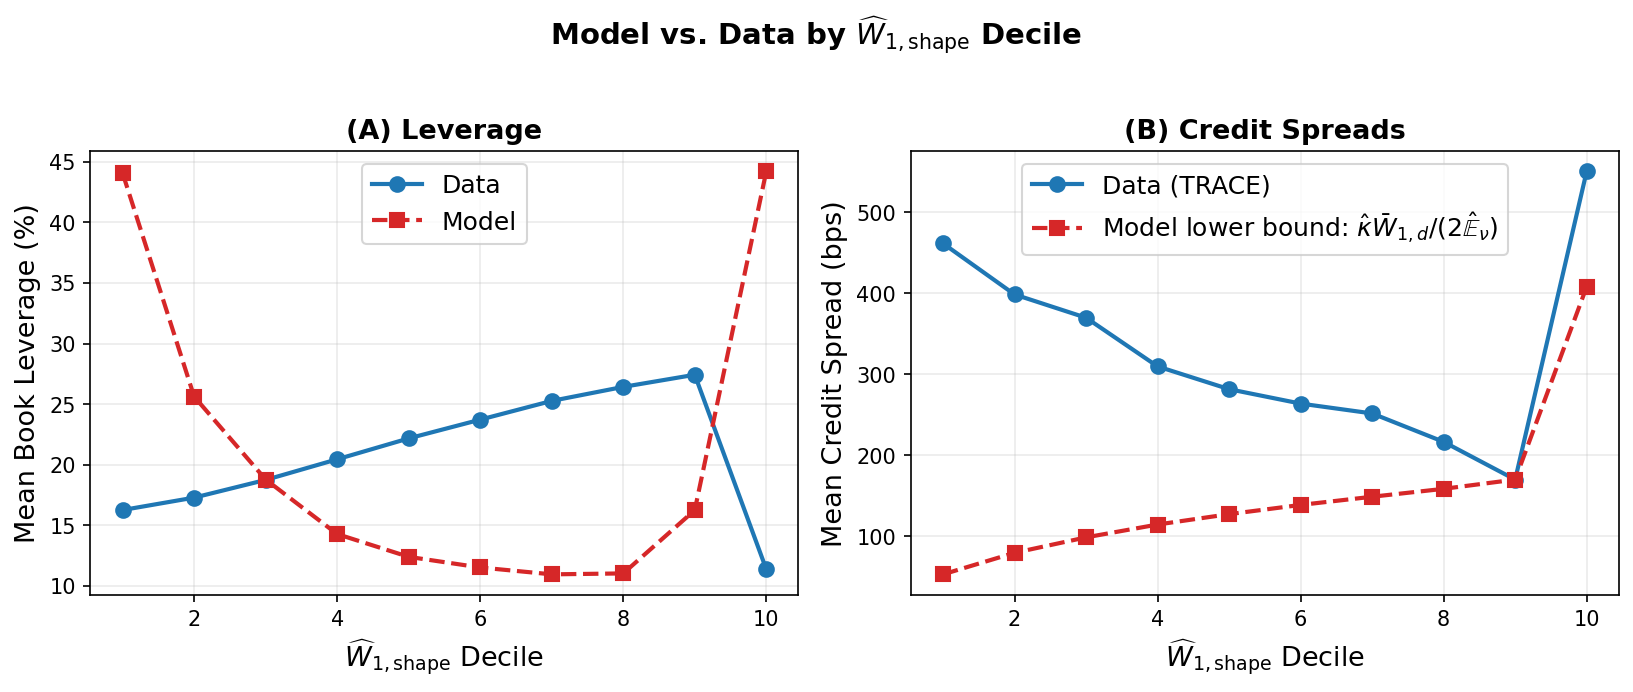
\includegraphics[width=\textwidth]{figures/fig_model_fit.pdf}
\caption{Model vs.\ Data: Leverage and Credit Spreads by $\widehat{W}_{1,\text{shape}}$ Decile.}
\label{fig:model_fit}
\footnotesize
\textit{Notes:} Decile 1 = lowest distributional mismatch; decile 10 = highest. Panel (A): mean book leverage (data vs.\ model). Panel (B): mean TRACE credit spread in basis points (2012--2024 subsample); the model line is the Proposition~\ref{prop:spreads} lower bound $\hat{\kappa}\,\bar{W}_{1,\text{shape},d}/(2\hat{\mathbb{E}}_\nu[Y])$, evaluated at the mean $\widehat{W}_{1,\text{shape}}$ of TRACE-matched firms in each decile. All bounds are satisfied ($\hat{\kappa}=0.104$, binding at decile~9).
\end{figure}

In the data, book leverage rises monotonically from decile 1 ($0.163$) to decile 9 ($0.274$) before falling sharply at decile 10 ($0.114$). The structural model predicts the opposite interior ordering: lowest mismatch firms (decile 1) borrow almost fully ($\hat{\lambda}^* \to 1$), giving high model leverage, while middle-decile firms face tighter participation constraints. The cross-decile $R^2$ is negative, reflecting that the composition effect dominates cross-sectional leverage variation.

The interior-decile mismatch arises from a cross-sectional composition effect: deciles 2--9 are dominated by large, investment-grade firms that are \emph{simultaneously} more diversified (lower distributional mismatch) \emph{and} more leveraged for reasons outside the model — covenant structure, credit ratings, and capital market access. The three-parameter structural model does not include these determinants, so the cross-decile level ordering is confounded by them. The model is intended as an analytically tractable benchmark that isolates the distributional mechanism under equal-mean conditions, not as a full cross-sectional leverage predictor competing with the Frank and Goyal (2009) horse race. The appropriate test of the model's prediction is the within-firm regression in Section~\ref{sec:results}, which controls for all time-invariant firm characteristics and thus removes the composition effect. The panel coefficient ($-0.163^{***}$, $t = -9.1$) is precisely the within-firm, mean-held-fixed prediction of Proposition~\ref{prop:leverage_wasserstein}.

The model's cross-decile fit would improve with additional structural parameters — for example, a composition-effect control for the fraction of firms with capital market access, or a dynamic extension with adjustment costs. These extensions are left for future work.
